\documentclass[a4paper]{article}

%% Language and font encodings
\usepackage[english]{babel}
\usepackage[utf8x]{inputenc}
\usepackage[T1]{fontenc}

%% Sets page size and margins
\usepackage[a4paper,top=3cm,bottom=2cm,left=3cm,right=3cm,marginparwidth=1.75cm]{geometry}

%% Useful packages
\usepackage{amsmath}
\usepackage{graphicx}
\usepackage[colorinlistoftodos]{todonotes}
\usepackage[colorlinks=true, allcolors=blue]{hyperref}

\title{Reporte de Actividad 6}
\author{Valenzuela Terán Jonás}

\begin{document}
\maketitle


\begin{center}
	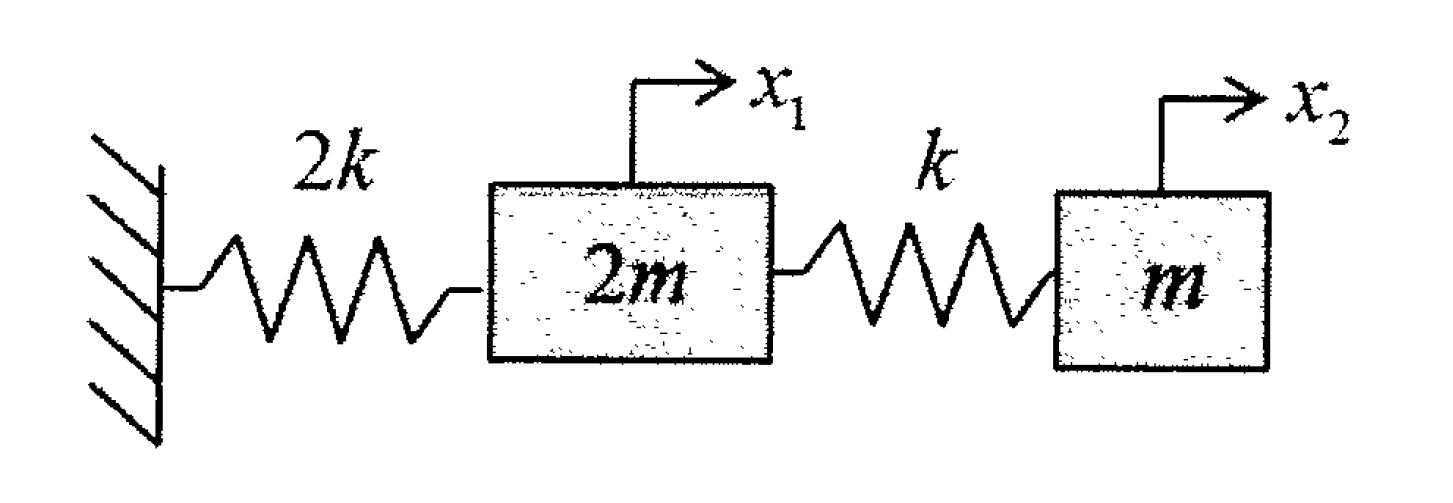
\includegraphics[height=4cm]{doblespring.png}
    
     Chris Olson - \textit{http://blog.gxsc.com/graphics\_systems\_solidnot/2014/02/behind-the-software-vibration-analysis.html}
\end{center}

\section{Introducción}

El objetivo de la actividad es aprender a modelar un fenómeno físico, en este caso, como ejemplo el sistema de doble resorte, a través de una simulación, hecha en el entorno que ha sido trabajado en clase últimamente, python en jupyter, pero esta vez en jupyter lab, que da a disposición un poco más de herramientas. Después, realizar distintas gráficas como las realizadas anteriormente para visualizar su comportamiento, y ver su confiabilidad mostrando el error relativo.


\section{Resumen de artículo: Coupled spring equations, pt. 1 y 2}

\subsection{Introducción}

La perspectiva general con la que se toma a las ecuaciones diferenciales esta cambiando mucho, de realizar técnicas para encontrar soluciones analíticas a visualizar y resolver numéricamente estas con las herramientas disponibles.

En el articulo, se trabaja con el problema de 2 resortes y 2 masas conectadas en serie, suponiendo que obedecen la Ley de Hooke. Esto introduce 2 ecuaciones diferencial linear de segundo orden. Hacer esto permite tener una interpretación física clara de la fase, amplitud, periodicidad, y la sensibilidad del sistema a las condiciones iniciales al introducir no linealidad.

\subsection{El modelo del doble resorte}

El modelo consiste en 2 resortes $k_1$ y $k_2$, y 2 masas $m_1$ y $m_2$ conectados en serie.

\subsubsection{Asumiendo la Ley de Hooke}

Suponiendo que  cumple la Ley de Hooke en el sistema, las fuerzas restauradoras producto de las elongaciones son de la forma $-k_1 l_1$ y $-k_2 l_2$ ($l$ siendo la elongación de cada resorte), la masa inferior solo siente la fuerza del resorte 2 $-k_2 (x_2 - x_1)$, donde $x_2 - x_1 = l_2$, mientras que la masa superior siente esta y la del resorte superior $-k_1 x_1$, donde $x_1 = l_1$. Escribimos las ecuaciones para las fuerzas de la forma:

\begin{center}
	$m_1 \ddot{x}_1 = - k_1 x_1 - k_2 (x_2 - x_1)$

	$m_2 \ddot{x}_2 = -k_2 (x_2 - x_1)$
\end{center}

Se tiene un par de ecuaciones diferenciales lineales de segundo orden, para obtener una ecuación de $x_1$ sin involucrar a $x_2$, se despeja de la ecuación:

\begin{center}
	$x_2 = -\frac{m_1 \ddot{x_1}}{k_2} + \frac{k_1 + k_2}{k_2} x_1$
\end{center}

una ecuación de segundo orden, la sustituimos en la segunda ecuación:

\begin{center}
$m_1 m_2 {x_1}^{(4)} + (m_2 k_1 + k_2 (m_1 + m_2)) \ddot{x}_1 + k_1 + k_2 x_1 = 0$
\end{center}

análogamente para $x_2$

\begin{center}
$m_1 m_2 {x_2}^{(4)} + (m_2 k_1 + k_2 (m_1 + m_2)) \ddot{x}_2 + k_1 + k_2 x_2 = 0$
\end{center}

Las 2 masas obedecen la misma ecuación, que solo necesita las 2 velocidades y posiciones iniciales para resolverla.  Podemos usar esta ecuación en la forma de 2 ecuaciones diferenciales de primer grado, con $v_1 = \ddot{x}_1$, $v_2 = \ddot{x}_2$.

\begin{center}
$v_1 = -\frac{k_1}{m_1} - \frac{k_2}{m_1} (x_1 - x_2)$

$v_2 = -\frac{k_2}{m_2} (x_2 - x_1)$
\end{center}

\subsubsection{Algunos ejemplos con masas iguales}

Se considera un modelo con $m_1 = m_2 = 1$, en el caso de no tener amortiguamiento, la ecuación característica es:

\begin{center}
$m^4 + (k_1 + 2 k_2) m_2 + k_1 k_2 = 0$
\end{center}

que tiene raíces: 

\begin{center}
$\pm \sqrt[]{-\frac{1}{2} k_1 - k_2 \pm \frac{1}{2} \sqrt[]{{k^2}_1 +4 {k^2}_2}}$
\end{center}


El ejemplo 2.1 plantea el sistema con $k_1 = 6$, $k_2 = 4$, y $(x_1(0),v_1(0),x_2(0),v_2(0)) = (1,0,2,0)$. Se obtiene, mediante lo desarrollado, la solución analítica:

\begin{center}
$x_1(t) = \cos \sqrt[]{2} t$

$x_2(t) = 2 \cos \sqrt[]{2} t$
\end{center}

Se observa que el movimiento para ambas masas es en fase, solo sus amplitudes son diferentes, las gráficas del movimiento y fase muestran patrones simples, estas se encontrarán en la sección \textit{Implementación en python (jupyter lab)}.

El ejemplo 2.2 tiene condiciones iniciales $k_1 = 6$, $k_2 = 4$, y $(x_1(0),v_1(0),x_2(0),v_2(0)) = (-2,0,1,0)$, que resulta en un movimiento completamente fuera de fase, las soluciones analíticas obtenidas, útiles en nuestro contexto para verificar el error de soluciones numéricas, son:

\begin{center}
$x_1(t) = -2 \cos 2 \sqrt[]{3} t$

$x_2(t) = \cos 2 \sqrt[]{3} t$
\end{center}

El ejemplo 2.3 tiene condiciones iniciales $k_1 = 0.4$, $k_2 = 1.808$, y $(x_1(0),v_1(0),x_2(0),v_2(0)) = (0.5,0,-0.5,0.7)$, aqui ocurre un movimiento más elaborado que los 2 anteriores, debido a que no entran completamente en fase o no fase, además, los valores de $k$ fueron seleccionados cuidadosamente para que ocurriera.

\subsubsection{Amortiguamiento}

Agregamos el amortiguamiento en las ecuaciones, introduciendo una fuerza que depende solamente de la velocidad de la masa, y coeficientes de fricción ${\delta}_1$ y ${\delta}_2$.

\begin{center}
	$m_1 \ddot{x}_1 = -{\delta}_1 v_1 - k_1 x_1 - k_2 (x_2 - x_1)$

	$m_2 \ddot{x}_2 = -{\delta}_2 v_2 -k_2 (x_2 - x_1)$
\end{center}

El ejemplo 2.4 introduce amortiguamiento, con condiciones iniciales $k_1 = 0.4$, $k_2 = 1.808$, ${\delta}_1 = 0.1$, ${\delta}_1 = 0.2$ y $(x_1(0),v_1(0),x_2(0),v_2(0)) = (1,0.5,2,0.5)$. Se observa como el movimiento es periódico pero pierde amplitud, sin embargo, la fase varía considerablemente.

\section{Implementación en python (jupyter lab)}

Se realizó una simulación de los ejemplos 2.1 al 2.4, generando puntos mediante una solución numérica y realizando gráficas los datos para producir figuras que muestren la posición contra tiempo, desplazamiento de m1 contra el de m2 y fase (desplazamiento contra velocidad). Todo esto mediante el entorno de programación jupyter lab, con lenguaje de programación Python y bibliotecas importadas para graficación y solución numérica.

\vspace{0.5cm}

\textit{Ejemplo 2.1}

\begin{center}
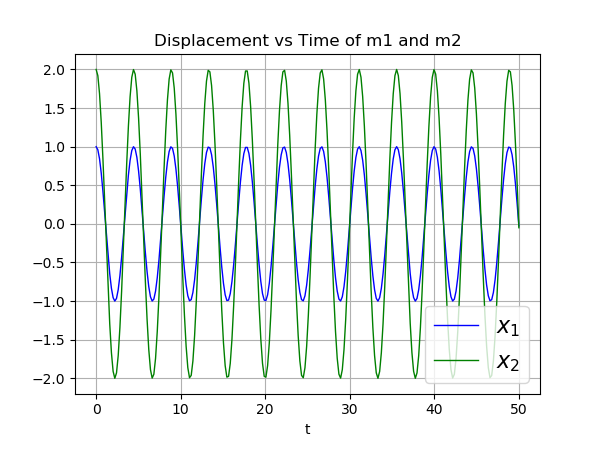
\includegraphics[height=6cm]{ejemplo2-1.png}

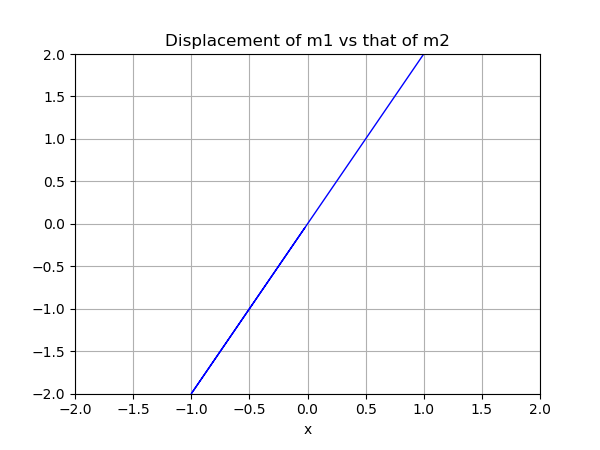
\includegraphics[height=6cm]{recta2-1.png}

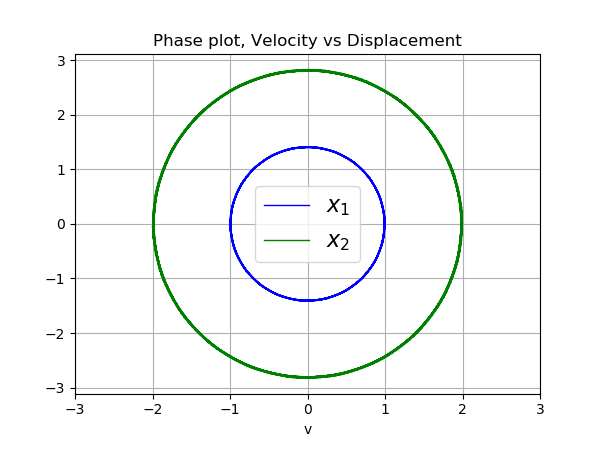
\includegraphics[height=6cm]{circulo2-1.png}

\end{center}

El error relativo de la solución numérica mostrada y de la solución analítica se ve mediante la siguiente gráfica:

\begin{center}
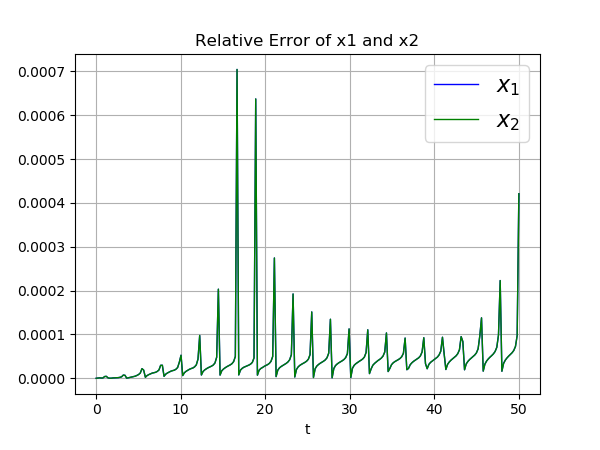
\includegraphics[height=6cm]{error2-1.png}
\end{center}

\textit{Ejemplo 2.2}

\begin{center}
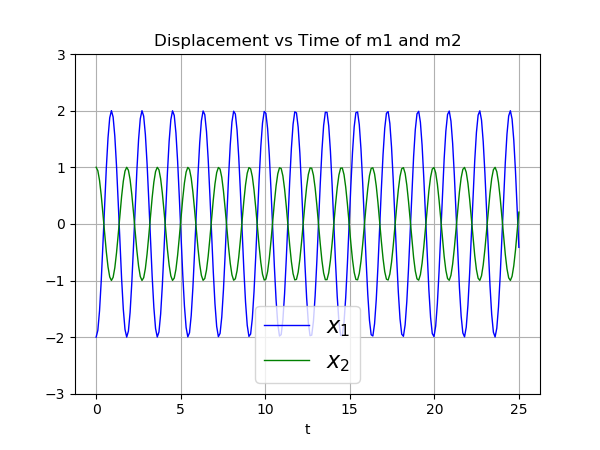
\includegraphics[height=6cm]{ejemplo2-2.png}

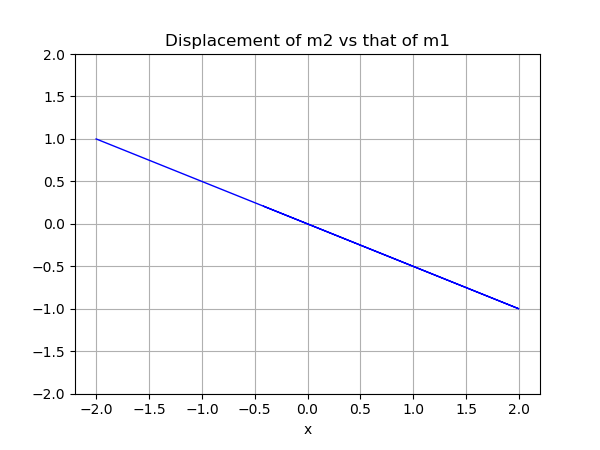
\includegraphics[height=6cm]{recta2-2.png}

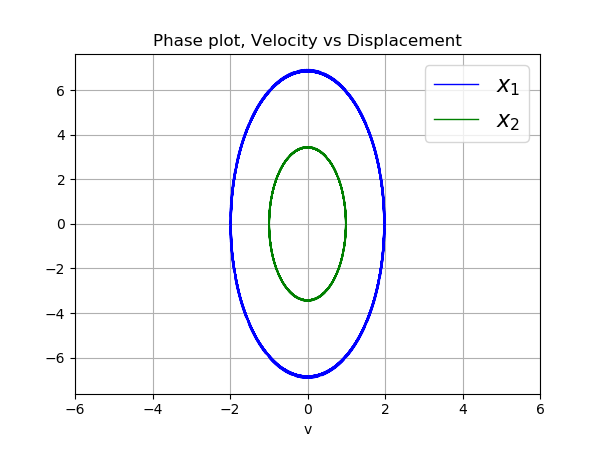
\includegraphics[height=6cm]{circulo2-2.png}
\end{center}

El error relativo de la solución numérica mostrada y de la solución analítica se ve mediante la siguiente gráfica:

\begin{center}
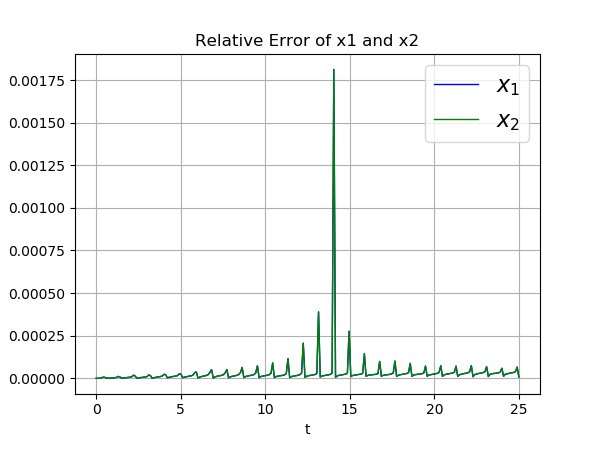
\includegraphics[height=6cm]{error2-2.png}
\end{center}

\textit{Ejemplo 2.3}

\begin{center}
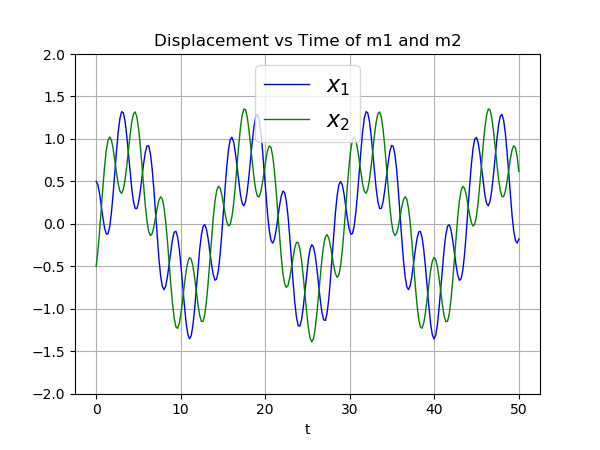
\includegraphics[height=6cm]{ejemplo2-3.png}

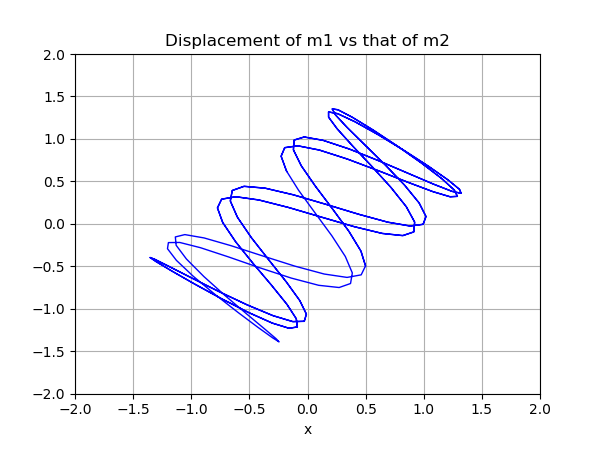
\includegraphics[height=6cm]{recta2-3.png}

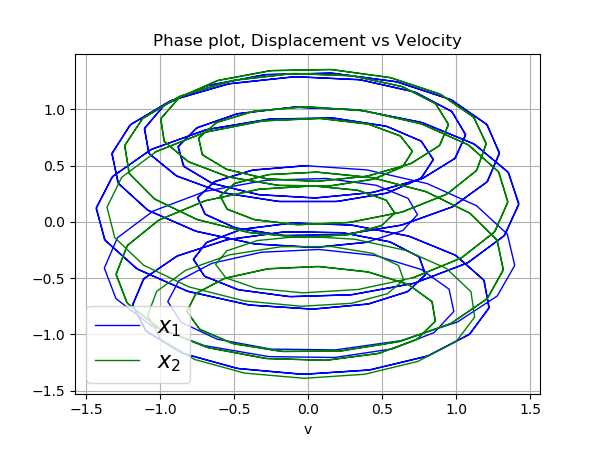
\includegraphics[height=6cm]{circulo2-3.png}
\end{center}

\textit{Ejemplo 2.4}

\begin{center}
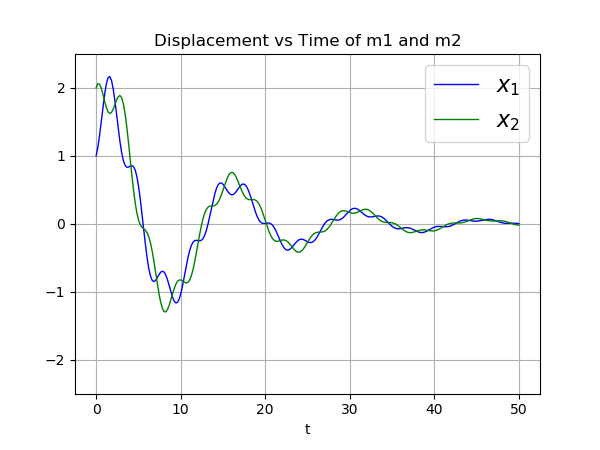
\includegraphics[height=6cm]{ejemplo2-4.png}

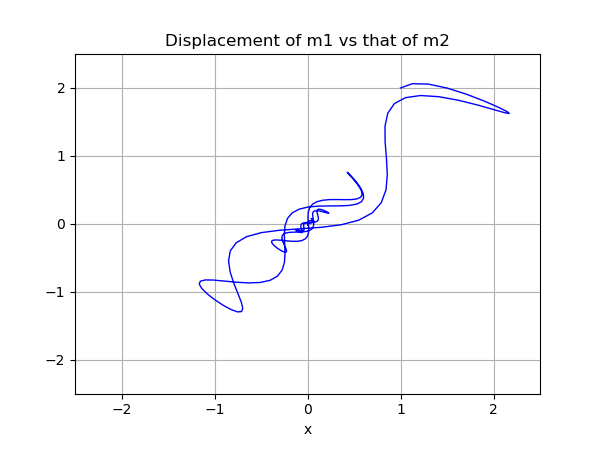
\includegraphics[height=6cm]{recta2-4.png}

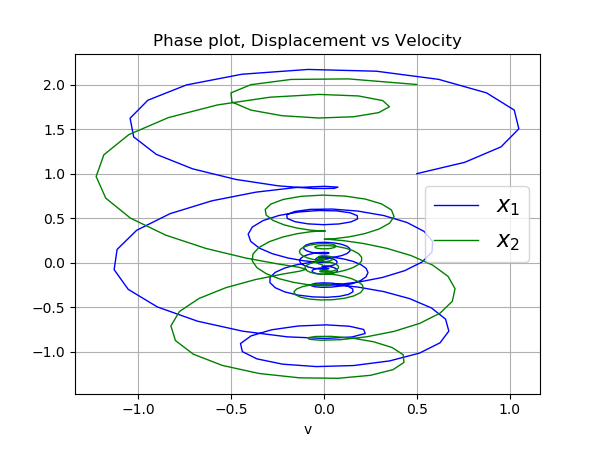
\includegraphics[height=6cm]{circulo2-4.png}
\end{center}

Para realizar cada ejemplo se siguen 3 pasos:

\begin{itemize}
\item Definir el modelo, declarando parámetros y especificando la función involucrada
\item Brindar valor a los parámetros, condiciones iniciales, y especificar el tiempo, tolerancia y número de puntos que se generan, escribiendo estos en un archivo.
\item Recuperar los resultados del archivo y especificar los ejes de lo que se desea graficar.
\end{itemize}


\section{Conclusiones}

Se encontró que el modelo si es efectivo en simular el sistema de doble resorte, aunque no produce resultados completamente confiables, esto es por la resolución numérica y discretización del movimiento, sin embargo, son datos y visualizaciones muy útiles para comprender el sistema.


\section{Bibliografía}

\begin{itemize}
\item SARAH DUNCAN GRAHAM. (2003). Coupled spring equations. 8 de Marzo, 2018, de University of Southern Mississippi Sitio web: 
\textit{http://math.oregonstate.edu/\~gibsonn/Teaching/MTH323-010S15/Supplements/coupled\_spring.pdf}


\item (2009). Coupled spring-mass system. 8 de marzo, 2018, de SciPy Cookbook Sitio web: 
\textit{http://scipy-cookbook.readthedocs.io/items/CoupledSpringMassSystem.html}
\end{itemize}



\section{Apéndice}

\begin{itemize}
\item     ¿En general te pareció interesante esta actividad de modelación matemática? ¿Qué te gustó mas? ¿Qué no te gustó?

Si me pareció muy interesante, se puede tener una mejor visualización del comportamiento del modelo físico.

\item     La cantidad de material te pareció ¿bien?, ¿suficiente?, ¿demasiado?

Opino que recibimos una cantidad buena de información, no poca ni demasiada.

\item     ¿Cuál es tu primera impresión de Jupyter Lab? 

Es más útil que jupyter notebook, ya que te permite mover las celdas, y ver los archivos producidos en el mismo lugar.

\item     Respecto al uso de funciones de SciPy, ¿ya habías visto integración numérica en tus cursos anteriores? ¿Cuál es tu experiencia?

Si, en Cálculo II, Fortran y Análisis Numérico, en general funcionan bien y rápidamente, pero nunca realizamos un modelo con muchas iteraciones.

\item     El tema de sistema de masas acopladas con resortes, ¿ya lo habías resuelto en tu curso de Mecánica 2?  

Fue mencionado, pero no estudiado.


\item     ¿Qué le quitarías o agregarías a esta actividad para hacerla más interesante y divertida? 

La dejaría como es actualmente.

\end{itemize}





\end{document}